\documentclass{beamer}
% \usepackage{etex}
\mode<presentation>{
  %\useinnertheme{rectangles}
  \useoutertheme{infolines}
  % \usecolortheme{crane}
  %\usecolortheme{rose}
}
%\usepackage{pdfpcnotes}
\newcommand{\pnote}[1] {}
\usepackage{multimedia}
\usepackage{tikz}
\usetikzlibrary{arrows.meta}
\usetikzlibrary{automata}
\usetikzlibrary{topaths}
\usetikzlibrary{shapes}
\usetikzlibrary{arrows}
\usetikzlibrary{decorations.markings}

\tikzstyle{place}=[circle,draw=black,inner sep=0mm, minimum size=6mm]
\tikzstyle{utility}=[diamond,draw=black,draw=blue!50,fill=blue!20,inner sep=0mm, minimum size=8mm]
\tikzstyle{select}=[rectangle,draw=black,draw=blue!50,fill=blue!20,inner sep=0mm, minimum size=6mm]
\tikzstyle{hidden}=[circle,draw=black,draw=green,fill=green!20,inner sep=0mm, minimum size=6mm]
\tikzstyle{transition}=[rectangle,draw=black!50,fill=black!20,thick]
\tikzstyle{observed}=[circle,draw=black,draw=blue!50,fill=blue!20,inner sep=0mm, minimum size=6mm]
\tikzstyle{someset}=[circle,draw=black,minimum size=8mm]
\tikzstyle{point}=[circle,draw=black,fill=black]

%% Use this for notes
%\usepackage{pgfpages}
%\setbeameroption{show notes on second screen}


% \usepackage[orientation=portrait, size=a4, scale=1.8,20pt]{beamerposter}
%\includeonly{rl_overview}
%% Pre-amble - commonly defined macros.

%% Packages
\usepackage{fixltx2e}
\usepackage{amsmath}
\usepackage{amsfonts}
\usepackage{amssymb}
\usepackage{amsbsy}
\usepackage{isomath}
\usepackage{amsthm}
\usepackage{dsfont}
%%\usepackage{theorem}
\usepackage{algorithm}
\usepackage{algorithmicx}
\usepackage{algpseudocode}
\usepackage{mathrsfs}
\usepackage{epsfig}
\usepackage{subcaption}
\usepackage{makeidx} 
\usepackage{colortbl}
\usepackage{enumerate}
\usepackage{multirow}
\usepackage{listings}
\usepackage{pgfplots}
\usepackage{fontawesome}
\newlength\fheight
\newlength\fwidth
\only<presentation>{
\setlength\fheight{\columnheight}
\setlength\fwidth{\columnwidth}
}
\only<article>{
\setlength\fheight{0.25\textheight}
\setlength\fwidth{0.5\textwidth}
}
\usepackage[sort&compress,comma,super]{natbib}
\def\newblock{} % To avoid a compilation error about a function \newblock undefined
\usepackage{hyperref}

\setbeamertemplate{theorems}[numbered] 
\mode<presentation>{
\theoremstyle{plain}
\newtheorem{assumption}{Assumption}
\theoremstyle{definition}
\newtheorem{exercise}{Exercise}
\theoremstyle{remark}
\newtheorem{remark}{Remark}
}

\numberwithin{equation}{section} 
\mode<article>{
  \theoremstyle{plain}
  % \newtheorem{assumption}{Assumption}[section]
  \newtheorem{lemma}{Lemma}[section]
  \newtheorem{theorem}{Theorem}[section]
  \newtheorem{corollary}{Corollary}[section]
  \theoremstyle{definition}
  \newtheorem{definition}{Definition}[section]
  \theoremstyle{remark}
  \newtheorem{remark}{Remark}[section]

  % \theoremstyle{plain} \newtheorem{remark}{Remark}[section]
  % \theoremstyle{plain} \newtheorem{definition}{Definition}[section]
  \theoremstyle{plain} \newtheorem{assumption}{Assumption}[section]
  
  %%% Examples %%%%
  \newtheoremstyle{example}  % Name
  {1em}       % Space above 
  {1em}       % Space below
  {\small}      % Body font
  {}          % Indent amount 
  {\scshape}  % Theorem head font
  {.}         % Punctuation after theorem head
  {.5em}      % Space after theorem head
  {}          % Theorem head spec
  \theoremstyle{example}
  \newtheorem{example}{Example}
  \newtheorem{exercise}{Exercise}

  \usepackage{framed}
  \usepackage[framemethod=tikz]{mdframed}
  \mdfsetup{%
    roundcorner=10pt}
  \renewenvironment{block}[1]
  {\begin{mdframed}[backgroundcolor=black!10,frametitle={#1}]}
    {\end{mdframed}}

  \renewenvironment{exampleblock}[1]
  {\begin{mdframed}[frametitle={\faGears{} #1}]}
    {\end{mdframed}}


  \renewenvironment{alertblock}[1]
  {\begin{mdframed}[backgroundcolor=red!20,frametitle={{\fontencoding{U}\fontfamily{futs}\selectfont\char 66\relax} #1}]}
    {\end{mdframed}}


  \newenvironment{theoryblock}[1]
  {\begin{mdframed}[backgroundcolor=yellow!20,frametitle={\Coffeecup #1}]}
    {\end{mdframed}}

  \newenvironment{exerciseblock}[1]
  {\begin{mdframed}[backgroundcolor=blue!10,frametitle={\faPencilSquareO{} #1}]}
    {\end{mdframed}}

  \newenvironment{groupactivity}[1]
  {\begin{mdframed}[backgroundcolor=cyan!20,frametitle={\faGroup{} #1}]}
    {\end{mdframed}}

  
}
%\theoremstyle{plain} \newtheorem{conjecture}{Conjecture}[section]
%\theoremstyle{plain} \newtheorem{theorem}{Theorem}[section]
%\theoremstyle{plain} \newtheorem{proposition}{Proposition}[section]
%\theoremstyle{plain} \newtheorem{lemma}{Lemma}[section]
%\theoremstyle{plain} \newtheorem{corollary}{Corollary}[section]


%\newenvironment{proof}[1][Proof]{\begin{trivlist}
%\item[\hskip \labelsep {\bfseries #1}]}{\end{trivlist}}
%\newcommand{\qed}{\nobreak \ifvmode \relax \else
%      \ifdim\lastskip<1.5em \hskip-\lastskip
%      \hskip1.5em plus0em minus0.5em \fi \nobreak
%      \vrule height0.5em width0.5em depth0.25em\fi}

\newcommand \indexmargin[1] {\marginpar{\emph{#1}}\index{#1}}
\newcommand \marginref[2] {\marginpar{\emph{#1}}\emph{#1}\index{#2}}
\newcommand \emindex[1] {\emph{#1}\marginpar{\emph{#1}}\index{#1}}


\newcommand \E {\mathop{\mbox{\ensuremath{\mathbb{E}}}}\nolimits}
\newcommand \hE {\hat{\mathop{\mbox{\ensuremath{\mathbb{E}}}}\nolimits}}
\renewcommand \Pr {\mathop{\mbox{\ensuremath{\mathbb{P}}}}\nolimits}
\newcommand \given {\mathrel{|}}
\newcommand \gvn {|}
\newcommand \eq {{=}}


%% Special characters
\newcommand\Reals {{\mathbb{R}}}
\newcommand\Naturals {{\mathbb{N}}} 
\newcommand\Simplex {\mathbold{\Delta}}

\newcommand \FB {{\mathfrak{B}}}
\newcommand \FD {{\mathfrak{D}}}
\newcommand \FF {{\mathfrak{F}}}
\newcommand \FM {{\mathfrak{M}}}
\newcommand \FK {{\mathfrak{K}}}
\newcommand \FJ {{\mathfrak{J}}}
\newcommand \FL {{\mathfrak{L}}}
\newcommand \FO {{\mathfrak{O}}}
\newcommand \FS {{\mathfrak{S}}}
\newcommand \FT {{\mathfrak{T}}}
\newcommand \FP {{\mathfrak{P}}}
\newcommand \FR {{\mathfrak{R}}}


\newcommand \CA {{\mathcal{A}}}
\newcommand \CB {{\mathcal{B}}}
\newcommand \CC {{\mathcal{C}}}
\newcommand \CD {{\mathcal{D}}}
\newcommand \CE {{\mathcal{E}}}
\newcommand \CF {{\mathcal{F}}}
\newcommand \CG {{\mathcal{G}}}
\newcommand \CH {{\mathcal{H}}}
\newcommand \CJ {{\mathcal{J}}}
\newcommand \CL {{\mathcal{L}}}
\newcommand \CM {{\mathcal{M}}}
\newcommand \CN {{\mathcal{N}}}
\newcommand \CO {{\mathcal{O}}}
\newcommand \CP {{\mathcal{P}}}
\newcommand \CQ {{\mathcal{Q}}}
\newcommand \CR {{\mathcal{R}}}
\newcommand \CS {{\mathcal{S}}}
\newcommand \CT {{\mathcal{T}}}
\newcommand \CU {{\mathcal{U}}}
\newcommand \CV {{\mathcal{V}}}
\newcommand \CW {{\mathcal{W}}}
\newcommand \CX {{\mathcal{X}}}
\newcommand \CY {{\mathcal{Y}}}
\newcommand \CZ {{\mathcal{Z}}}

\newcommand \BA {{\mathbb{A}}}
\newcommand \BI {{\mathbb{I}}}
\newcommand \BS {{\mathbb{S}}}

\newcommand \bx {{\vectorsym{x}}}
\newcommand \by {{\vectorsym{y}}}
\newcommand \bu {{\vectorsym{u}}}
\newcommand \bw {{\vectorsym{w}}}
\newcommand \ba {{\vectorsym{a}}}
\newcommand \bc {{\vectorsym{c}}}
\newcommand \bz {{\vectorsym{z}}}
\newcommand \bq {{\vectorsym{q}}}
\newcommand \bat {{\vectorsym{a}_t}}
\newcommand \bh {{\vectorsym{h}}}
\newcommand \bo {{\vectorsym{o}}}
\newcommand \bp {{\vectorsym{p}}}
\newcommand \bs {{\vectorsym{s}}}
\newcommand \br {{\vectorsym{r}}}

\newcommand \SA {\mathscr{A}}
\newcommand \SB {\mathscr{B}}
\newcommand \SC {\mathscr{C}}
\newcommand \SF {\mathscr{F}}
\newcommand \SG {\mathscr{G}}
\newcommand \SH {\mathscr{H}}
\newcommand \SJ {\mathscr{J}}
\newcommand \SL {\mathscr{L}}
\newcommand \SP {\mathscr{P}}
\newcommand \SR {\mathscr{R}}
%%\newcommand \SS {\mathscr{S}}
\newcommand \ST {\mathscr{T}}
\newcommand \SU {\mathscr{U}}
\newcommand \SV {\mathscr{V}}
\newcommand \SW {\mathscr{W}}

\newcommand \hM {\widehat{M}}

\newcommand \KL[2] {\mathbb{D}\left( #1 \| #2 \right)}


%\newcommand \p {\partial}

\newcommand \then{\Rightarrow}
\newcommand \defn {\mathrel{\triangleq}}
%\newcommand \StateSet {{\CQ}}


%% Commands

\newcommand \argmax{\mathop{\rm arg\,max}}
\newcommand \argmin{\mathop{\rm arg\,min}}
\newcommand \dtan{\mathop{\rm dtan}}
\newcommand \sgn{\mathop{\rm sgn}}
\newcommand \trace{\mathop{\rm tr}}

\newcommand \onenorm[1]{\left\|#1\right\|_1}
\newcommand \pnorm[2]{\left\|#1\right\|_{#2}}
\newcommand \inftynorm[1]{\left\right\|#1\|_\infty}
\newcommand \norm[1]{\left\|#1\right\|}

%%\newcommand \defn {\triangleq}
%%\newcommand \defn {\equiv}
%%\newcommand \defn {\coloneq}
%%\newcommand \defn {\stackrel{\text{\tiny def}}{=}}
%%\newcommand \defn {\stackrel{\text{def}}{\hbox{\equalsfill}}}

\DeclareMathAlphabet{\mathpzc}{OT1}{pzc}{m}{it}

\newcommand \Normal {\mathop{\mathpzc{N}}\nolimits}
\newcommand \Poisson {\mathop{\mathpzc{Poisson}}\nolimits}
\newcommand \Multinomial {\mathop{\mathpzc{Multinomial}}\nolimits}
\newcommand \Dirichlet {\mathop{\mathpzc{Dirichlet}}\nolimits}
\newcommand \Student {\mathop{\mathpzc{Student}}\nolimits}
\newcommand \Bernoulli {\mathop{\mathpzc{Bernoulli}}\nolimits}
\newcommand \BetaDist   {\mathop{\mathpzc{Beta}}\nolimits}
\newcommand \Singular   {\mathop{\mathpzc{D}}\nolimits}
\newcommand \GammaDist {\mathop{\mathpzc{Gamma}}\nolimits}
\newcommand \Softmax{\mathop{\mathpzc{Softmax}}\nolimits}
\newcommand \Exp{\mathop{\mathpzc{Exp}}\nolimits}
\newcommand \Uniform{\mathop{\mathpzc{Unif}}\nolimits}
\newcommand \Laplace {\mathop{\mathpzc{Laplace}}\nolimits}

\newcommand \Param {\Theta}
\newcommand \param {\theta}
\newcommand \vparam {\vectorsym{\theta}}
\newcommand \mparam {\matrixsym{\Theta}}
\newcommand \Hyperparam {\Phi}
\newcommand \hyperparam {\phi}
\newcommand \family {\mathcal{F}}
\newcommand{\ie}{\emph{i.e.}~}
\newcommand{\eg}{\emph{e.g.}~}
\newcommand{\etal}{\emph{et al.}~}
\newcommand{\constg}{}
\newcommand{\Bel}{\mathcal{B}}
\newcommand \Bay {\ensuremath{\mathscr{B}}}
\newcommand \Adv {\ensuremath{\mathscr{A}}}

\newcommand \step {\eta}

\newcommand \Borel[1] {\FF(#1)}
\newcommand \Probs[1] {\FM(#1)}


\newcommand \pol {\pi}
\newcommand \Pol {\Pi}
\newcommand \mdp {\mu}
\newcommand \MDP {\CM}
\newcommand \meanMDP {{\bar{\mdp}_\xi}}

\newcommand {\msqr} {\vrule height0.33cm width0.44cm}
\newcommand {\bsqr} {\vrule height0.55cm width0.66cm}

\newcommand\ind[1]{\mathop{\mbox{\ensuremath{\mathbb{I}}}}\left\{#1\right\}}
\newcommand\Ind{\mbox{\bf{I}}}

\newcommand\dd{\,\mathrm{d}}

\newcommand \seq[2]{#1^{#2}}
\newcommand \pseq[3]{#1_{#2}^{#3}}
\newcommand \sam[2]{#1^{(#2)}}
\newcommand \transpose[1] {#1^\top}
\newcommand\set[1] {\left\{#1\right\}}
\newcommand\tuple[1] {\left\langle #1\right\rangle}
\newcommand\cset[2] {\left\{#1 ~\middle|~ #2\right\}}
\newcommand \ceil[1]{\left\lceil #1 \right\rceil}





\newcommand{\indep}{\mathrel{\text{\scalebox{1.07}{$\perp\mkern-10mu\perp$}}}}


\newcommand \eqlike {\eqsim}
\newcommand \gtlike {\succ}
\newcommand \ltlike {\prec}
\newcommand \gelike {\succsim}
\newcommand \lelike {\precsim}

\newcommand \eqpref {\eqsim^*}
\newcommand \gtpref {\succ^*}
\newcommand \ltpref {\prec^*}
\newcommand \gepref {\succsim^*}
\newcommand \lepref {\precsim^*}

\newcommand \util {U}
\newcommand \BUtil {U^*}
\newcommand \MUtil {\matrixsym{U}}
\newcommand \risk {\sigma}
\newcommand \Brisk {\sigma^*}
\newcommand \Loss {\ell}
\newcommand \Regret {L}
\newcommand \regret {\ell}
\newcommand \Reward {\SR}
\newcommand \reward {r}
\newcommand \vreward {\vectorsym{r}}
\newcommand \Rew {\rho}
\newcommand \boutcome {\vectorsym{\omega}}
\newcommand \outcome {\omega}
\newcommand \Outcome {\Omega}
\newcommand \act {a}
\newcommand \Act {\CA}
\newcommand \decision {a}
\newcommand \Decision {\mathcal{A}}
\newcommand \dec {\delta}
\newcommand \Dec {\mathscr{D}}


\newcommand {\MH} {\matrixsym{H}}

\newcommand \alg {\lambda}
\newcommand \Alg {\Lambda}
\newcommand \KNN {\textsc{k-NN}}

\newcommand \model {\mu}
\newcommand \MAP {\model_{\textrm{MAP}}}
\newcommand \Model {\CM}
\newcommand \Datasets {\CD}
\newcommand \Data {D}
\newcommand \Training {D_T}
\newcommand \Holdout {D_H}
\newcommand \Testing {D^*}
\newcommand \error {\epsilon}
\newcommand \obs {x}
\newcommand \Obs {\CX}
\newcommand \Att {\CA}
\newcommand \att {a}
\newcommand \attv {v}
\newcommand \Attv {\CV}
\newcommand \cls {y}
\newcommand \Cls {\CY}
\newcommand \Entropy {\mathbb{H}}
\newcommand \Gain {\mathbb{G}}


\newcommand \IDThree {\texttt{ID3}}

\newcommand \nactions {A}
\newcommand \nclasses {C}
\newcommand \nstates{S}
\newcommand \nobservations {N}
\newcommand \ndata{T}

\newcommand \figwidth {0.6\textwidth}
\newcommand \figheight {0.4\textwidth}

\newcommand \eye {\matrixsym{I}}
\newcommand \MA {\matrixsym{A}}
\newcommand \MC {\matrixsym{C}}
\newcommand \MX {\matrixsym{X}}
\newcommand \MR {\matrixsym{R}}
\newcommand \MY {\matrixsym{Y}}
\newcommand \MB {\matrixsym{B}}
\newcommand \MV {\matrixsym{V}}
\newcommand \MW {\matrixsym{W}}
\newcommand \MP {\matrixsym{P}}
\newcommand \MZ {\matrixsym{Z}}

\newcommand \vg {\vectorsym{\gamma}}
\newcommand \vp {\vectorsym{p}}
\newcommand \vs {\vectorsym{s}}
\newcommand \vx {\vectorsym{x}}
\newcommand \vr {\vectorsym{r}}
\newcommand \vm {\vectorsym{m}}
\newcommand \vb {\vectorsym{b}}
\newcommand \vt {\vectorsym{\theta}}

\newcommand \pn[1] {\vx_{[#1]}}

\newcommand \basis {f}
\newcommand \bel {\beta}
\newcommand \hyper {\omega}
\newcommand \mbel {\bel^D}
\newcommand \pbel {\bel^C}

\newcommand \pmean {\matrixsym{M}}
\newcommand \pcov {\matrixsym{C}}
\newcommand \pwish {\matrixsym{W}}
\newcommand \porder {n}

\newcommand \Syx {\matrixsym{\Sigma}_{yx}}
\newcommand \Sxx {\matrixsym{\Sigma}_{xx}}
\newcommand \Syy {\matrixsym{\Sigma}_{yy}}
\newcommand \Symx {\matrixsym{\Sigma}_{y\mid x}}

\newcommand \trans {\matrixsym{P}}
\newcommand \ident {\matrixsym{I}}

\newcommand \noise {\vectorsym{\varepsilon}}

\newcommand \pt {p_t}


\newcommand \CSet {G}
\newcommand \Parent[1] {\mathfrak{P}(#1)}
\newcommand \Children[1] {\mathfrak{C}(#1)}
\newcommand \Ancestors[1] {\mathfrak{A}(#1)}
\newcommand \Descendants[1] {\mathfrak{D}(#1)}
\newcommand \metric[2] {\nu(#1, #2)}
\newcommand \zooming {\zeta}
\newcommand \depth[1] {d(#1)}

\newcommand \sensitivity[1] {\mathbb{L}\left(#1\right)}
\newcommand \disc {\gamma}
\newcommand \Value {V}
\newcommand \val {\vectorsym{v}}
\newcommand \Vals {\mathcal{V}}
\newcommand \qval {\vectorsym{q}}
\newcommand \Qvals {\mathcal{Q}}
\newcommand \blm {\mathscr{L}}
\newcommand \tdm {\mathscr{D}}
\newcommand \pim {\mathscr{B}}



\newcommand \dist[2]{D\left(#1 ~\middle\|~ #2\right)}

\newcommand \Ae {A_\epsilon^\hist}

\newcommand \lrdist[2]{d_{lr}(#1, #2)}
\newcommand \xdistChar{\rho}
\newcommand \xdist[2]{\xdistChar(#1, #2)}
\newcommand \pdist[2]{\kappa(#1, #2)}
\newcommand{\constScale}{\omega}
\newcommand{\constScaleB}{\kappa}

\newcommand \fields[1]{\sigma(#1)}

\newcommand \hist {h}

\newcommand \abs[1] {\left|#1\right|}

\newcommand{\errorband}[5][]{ % x column, y column, error column, optional argument for setting style of the area plot
\pgfplotstableread[col sep=comma, skip first n=2]{#2}\datatable
% Lower bound (invisible plot)
\addplot [draw=none, stack plots=y, forget plot] table [
x={#3},
y expr=\thisrow{#4}-\thisrow{#5}
] {\datatable};

% Stack twice the error, draw as area plot
\addplot [draw=none, fill=gray!40, stack plots=y, area legend, #1] table [
x={#3},
y expr=2*\thisrow{#5}
] {\datatable} \closedcycle;

% Reset stack using invisible plot
\addplot [forget plot, stack plots=y,draw=none] table [x={#3}, y expr=-(\thisrow{#4}+\thisrow{#5})] {\datatable};
}


%%% macros to make things smalller
% For comparison, the existing overlap macros:
% \def\llap#1{\hbox to 0pt{\hss#1}}
% \def\rlap#1{\hbox to 0pt{#1\hss}}
\def\clap#1{\hbox to 0pt{\hss#1\hss}}
\def\mathllap{\mathpalette\mathllapinternal}
\def\mathrlap{\mathpalette\mathrlapinternal}
\def\mathclap{\mathpalette\mathclapinternal}
\def\mathllapinternal#1#2{%
\llap{$\mathsurround=0pt#1{#2}$}}
\def\mathrlapinternal#1#2{%
\rlap{$\mathsurround=0pt#1{#2}$}}
\def\mathclapinternal#1#2{%
\clap{$\mathsurround=0pt#1{#2}$}}


\usepackage{tikz}
\usepackage{tikzsymbols}
%\usetikzlibrary{external}
%\tikzexternalize[prefix=tikz/]
\usepackage{gnuplot-lua-tikz}


\usetikzlibrary{automata}
\usetikzlibrary{topaths}
\usetikzlibrary{shapes}
\usetikzlibrary{arrows}
\usetikzlibrary{decorations.markings}
\usetikzlibrary{intersections}
\usetikzlibrary{backgrounds}
\usetikzlibrary{positioning}


\tikzstyle{utility}=[diamond,draw=black,draw=blue!50,fill=blue!10,inner sep=0mm, minimum size=8mm]
\tikzstyle{select}=[rectangle,draw=black,draw=blue!50,fill=blue!10,inner sep=0mm, minimum size=6mm]
\tikzstyle{hidden}=[dashed,draw=black,fill=red!10]
\tikzstyle{RV}=[circle,draw=black,draw=blue!50,fill=blue!10,inner sep=0mm, minimum size=6mm]
\tikzstyle{place}=[circle,draw=black,draw=blue!50,fill=blue!20,inner sep=0mm, minimum size=9mm]
\tikzstyle{transition}=[rectangle,draw=black!50,fill=black!20,thick]
\tikzstyle{observed}=[circle,draw=black,draw=blue!50,fill=blue!10,inner sep=0mm, minimum size=6mm]
\tikzstyle{someset}=[circle,draw=black,minimum size=8mm]

\tikzstyle{known}=[rectangle,draw=green!50,fill=green!20,thick]
\tikzstyle{queried}=[rectangle,draw=blue!50,fill=blue!20,thick]
%\tikzstyle{transition}=[rectangle,draw=black!50,fill=black!20,thick]

\tikzstyle{thickarrow}=[->, >=latex, line width=15pt, green!50]
\tikzstyle{medarrow}=[->, >=latex,  line width=5pt]
\tikzstyle{arrow}=[->,>=triangle 60]

\tikzset{every picture/.style={
    line width=1
  }
}

\definecolor{dark-green}{rgb}{0,0.5,0}




\definecolor{mycolor1}{rgb}{0.00000,0,1}%
\definecolor{mycolor2}{rgb}{1,0,0}%
\setlength \fwidth {0.75\textwidth}

\title{Digital Skills}
\subtitle{Data Collection, Visualisation and Modelling}
\author[C. Dimitrakakis]{Christos Dimitrakakis}
\institute{University of Neuchatel}
\date{27 September 2022}
\begin{document}

\usebackgroundtemplate{
  \tikz[overlay,remember picture] \node[opacity=0.3, at=(current page.center)] {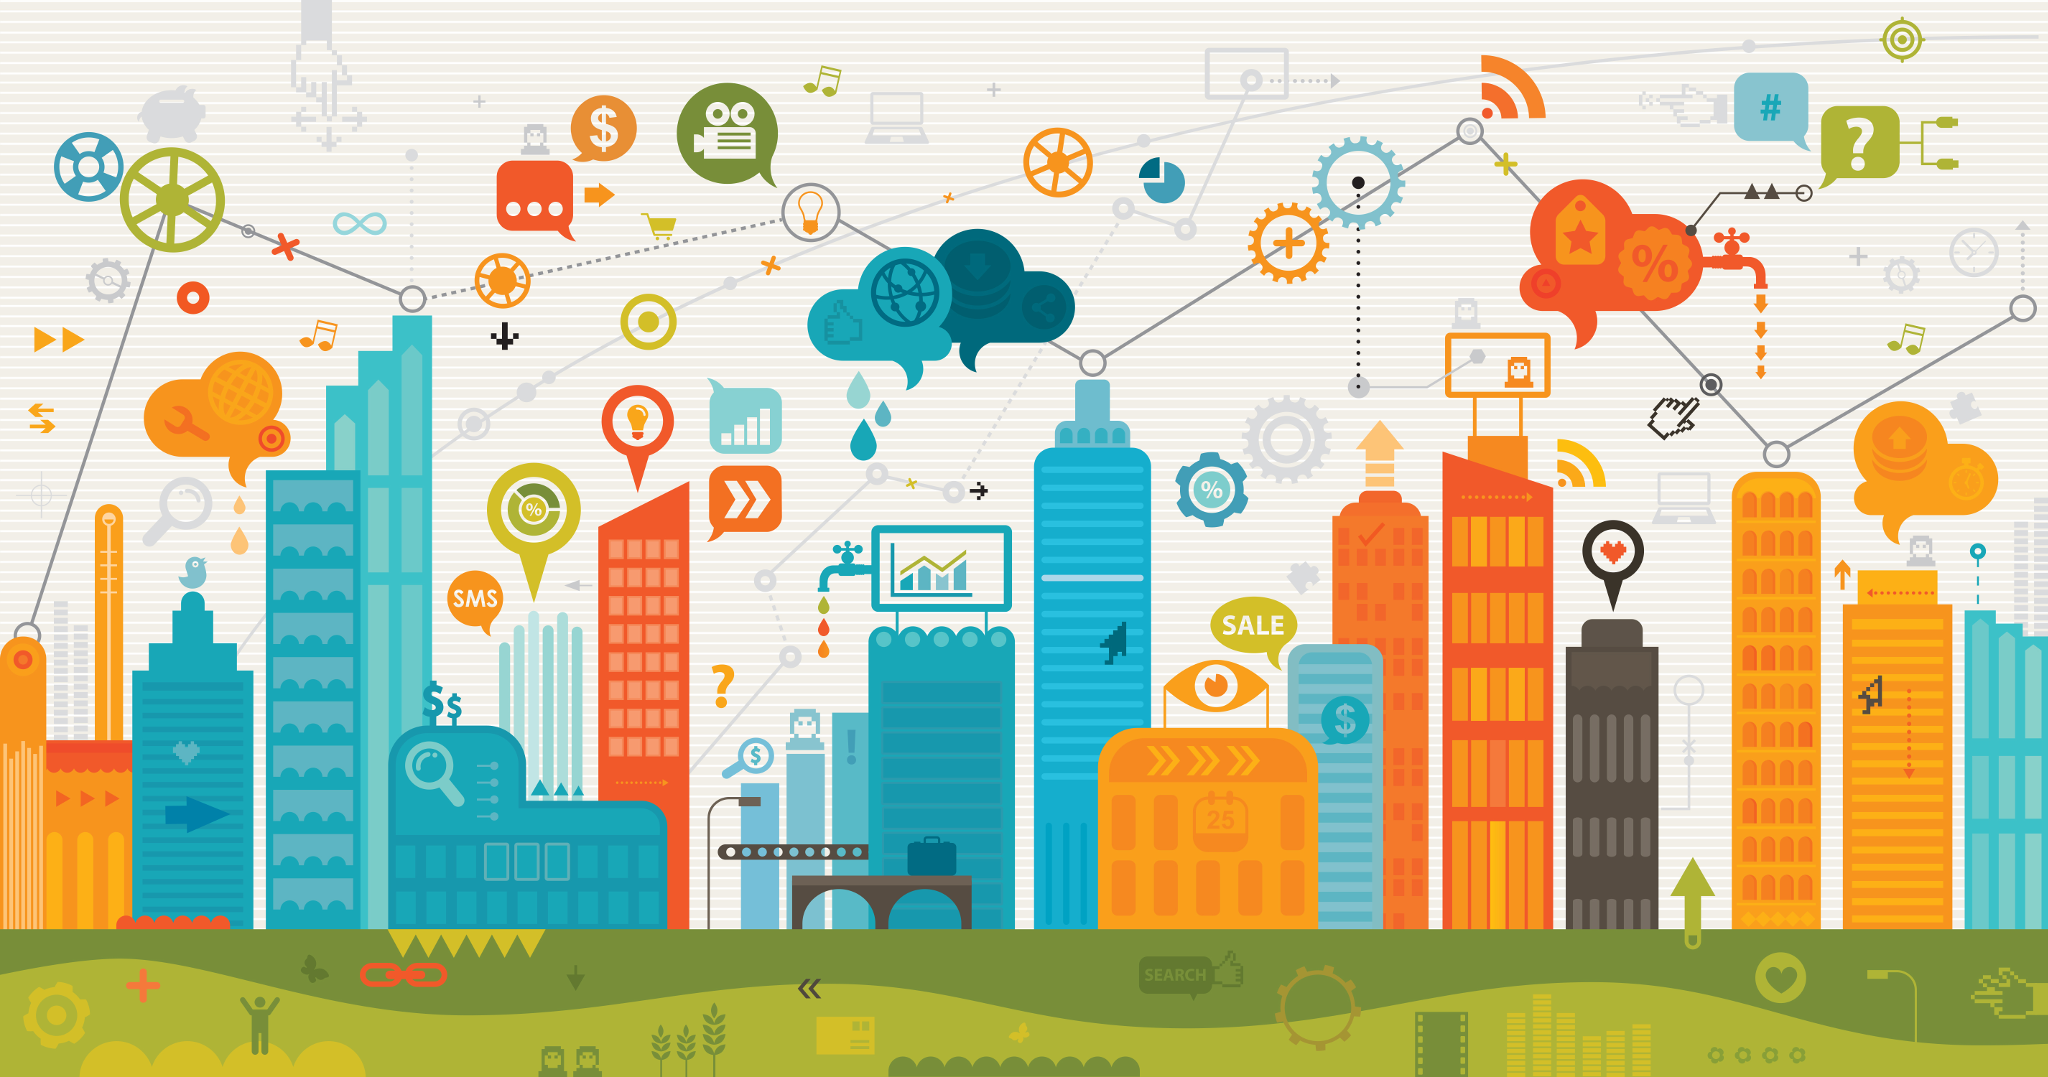
\includegraphics{figures/IoT.png}};
}
\begin{frame}
  \titlepage
\end{frame}
\usebackgroundtemplate{}


% data analysis is just a minor part of machine learning
\section{Introduction}
\include{ml_science}

\section{Data science overview}


\begin{frame}
  \centering
  \begin{columns}
    \begin{column}{0.5\textwidth}
      \centering
      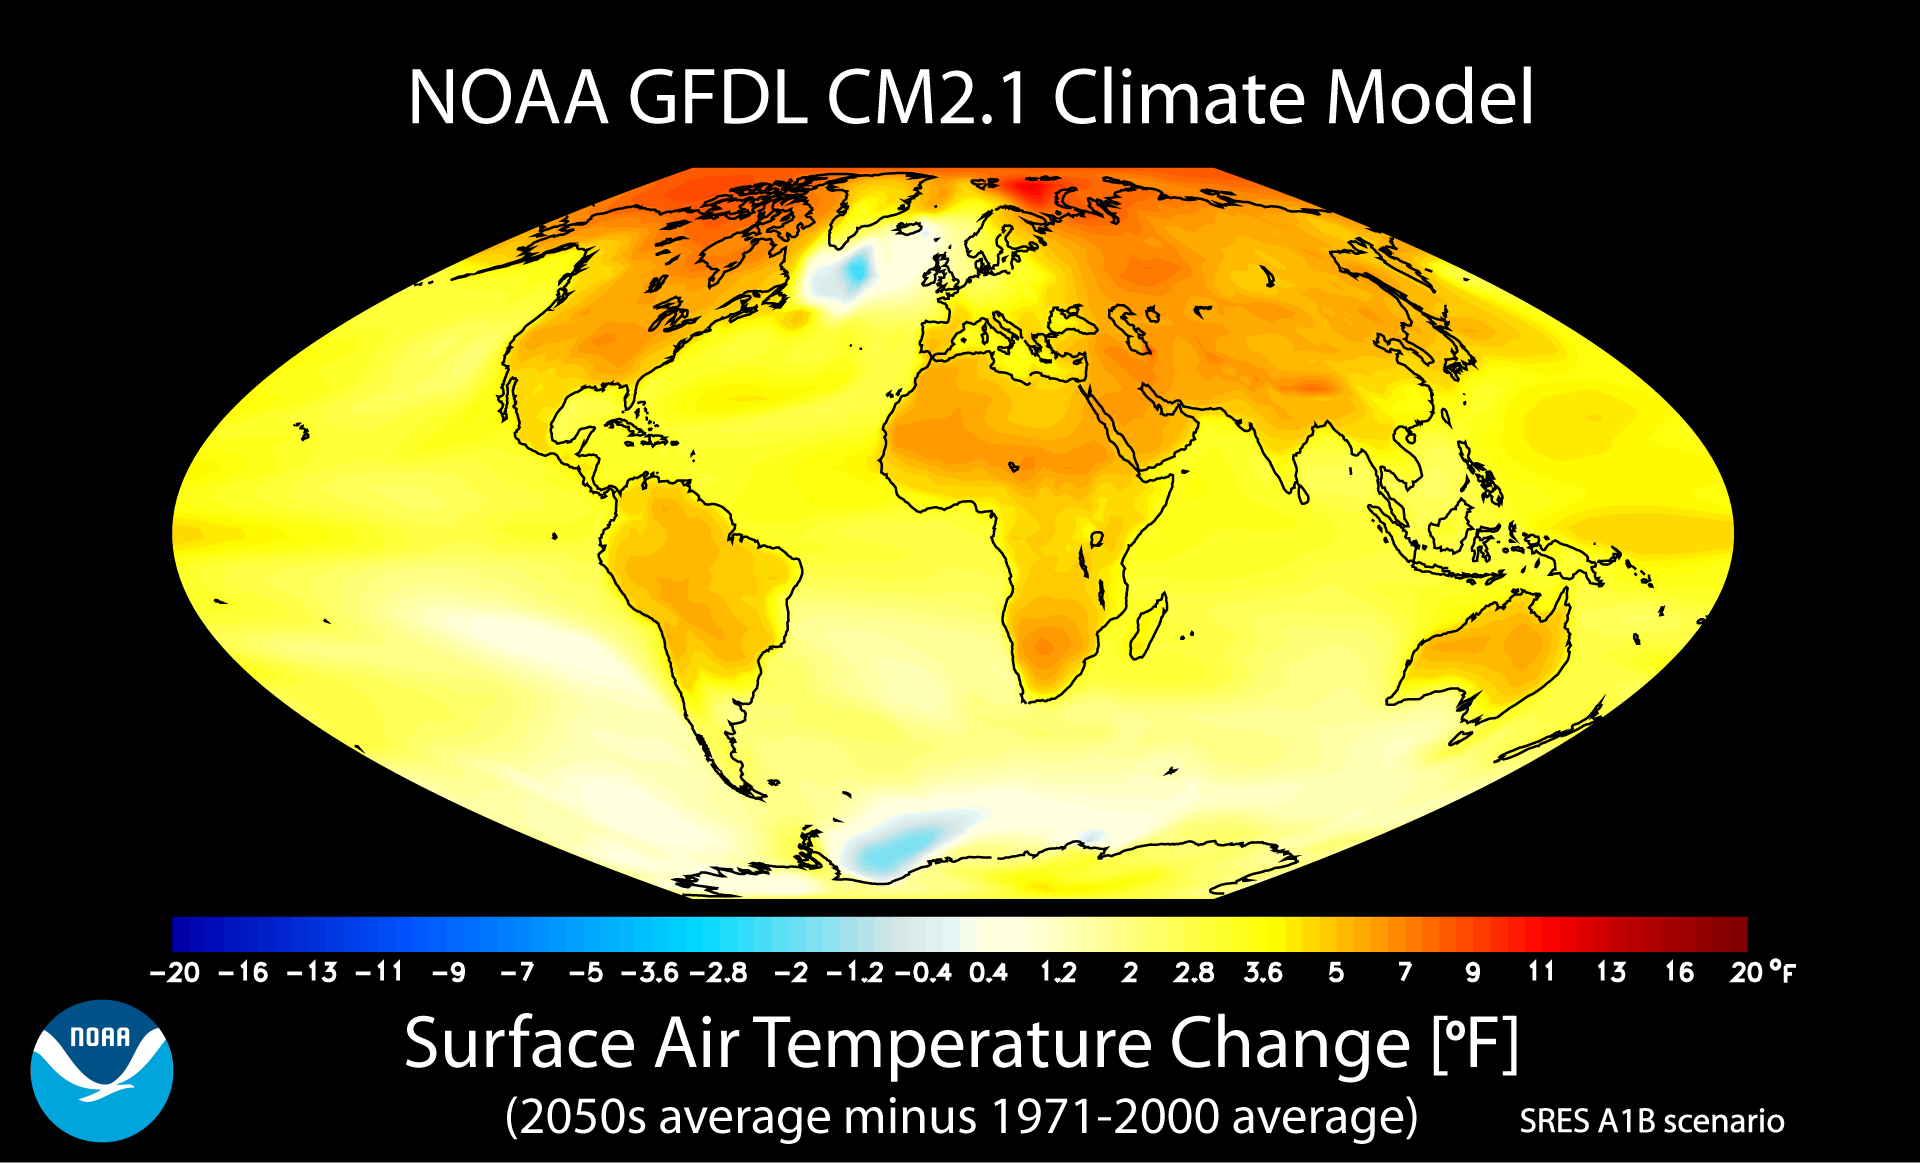
\includegraphics[width=0.8\columnwidth]{figures/gfdl_2050.png}
      \\
      \textbf{Climatology}
      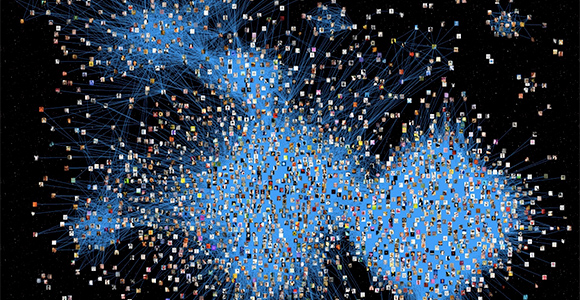
\includegraphics[width=0.8\columnwidth]{figures/networks-2.jpg}
      \\
      \textbf{Humanities}
      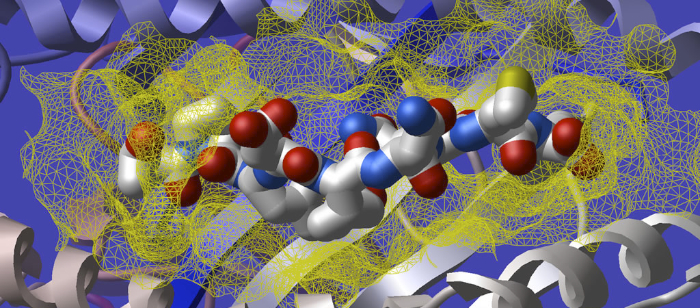
\includegraphics[width=0.8\columnwidth]{figures/protein.jpg}\\
      \textbf{Biology}
    \end{column}
    \begin{column}{0.5\textwidth}
      \centering
      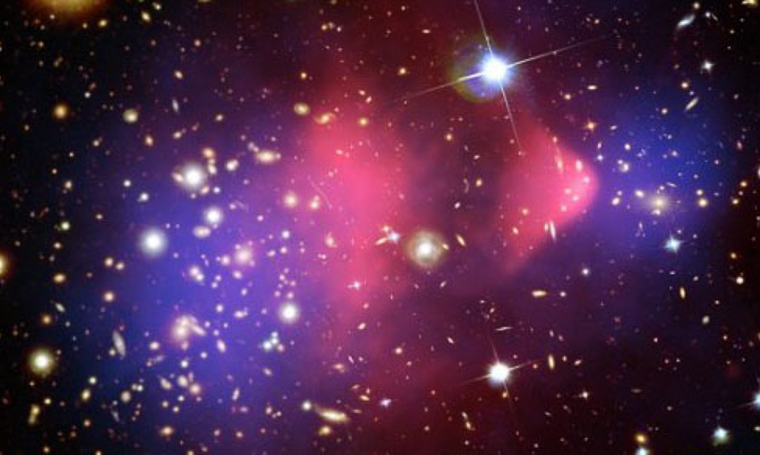
\includegraphics[width=0.8\columnwidth]{figures/dark_matter.jpg}
      \\
      \textbf{Cosmology}
      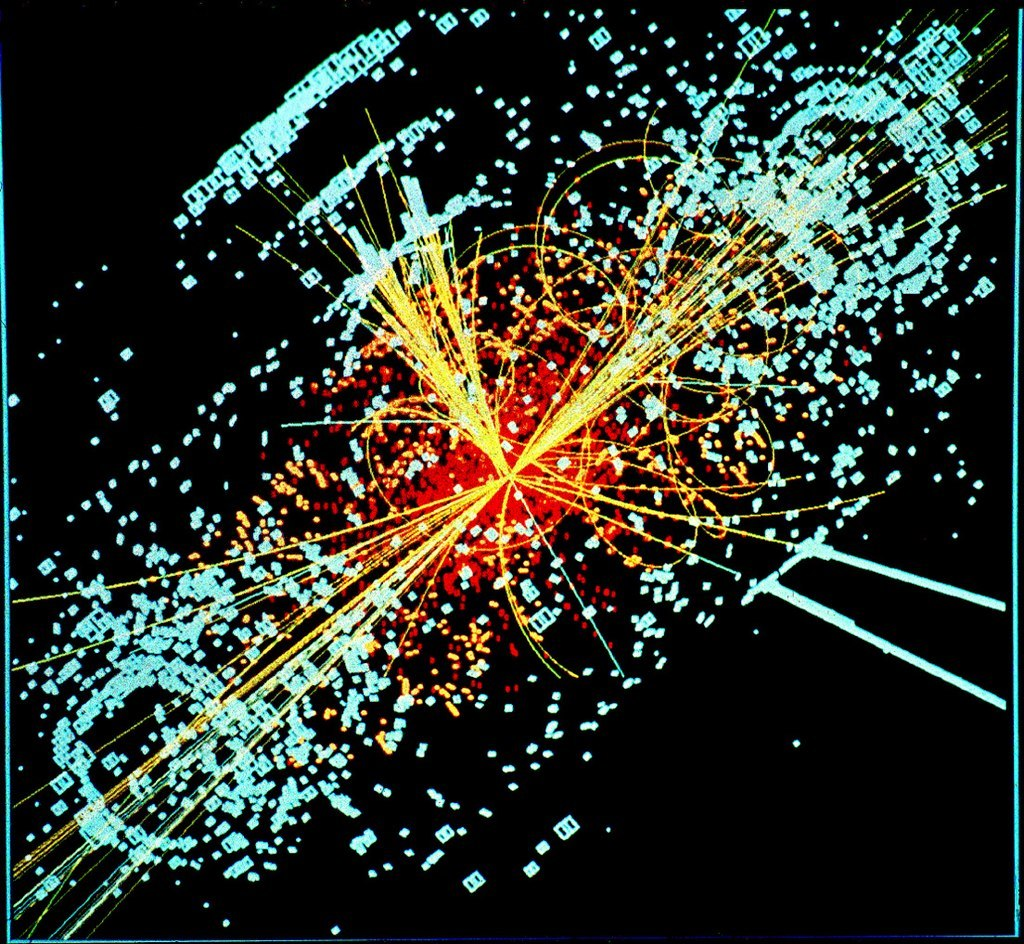
\includegraphics[width=0.8\columnwidth]{figures/higgs.jpg}      \\
      \textbf{Nuclear physics}
    \end{column}
  \end{columns}
  \only<2>{
    \begin{tikzpicture}[remember picture,overlay]
      \draw[fill=black,opacity=0.75] 
      (current page.north east) rectangle (current page.south west);
      \node[align=center] at (current page.center) {
        {\Huge \alert{Reproducibility, Data Collection}}
      };
    \end{tikzpicture}}
  \pnote{
    Science is a classic example where we must use data to understand how the world works, essentially creating a belief about which models are true. In some domains, like climatology, these models are complex simulators with many parameters. These and are validated using data from satellites and sea buoys. In others we can also general machine learning models such as Gaussian processes, used to map the distribution of dark matter in the universe, or neural networks, used with a lot of success recently to model protein folding.

However, we always face the problem data collection. Given what we believe right now, what data should we collect, what experiment should we perform, in order to increase our understanding of the world? So e.g. should we use robotic submarines to monitor deep sea temperatures? Should we generate our own news stories in a social network in order to study the interaction between communities and news propagation? 
   }
\end{frame}




\begin{frame}
  \frametitle{Can machines learn from data?}
  \begin{center}
    \only<1>{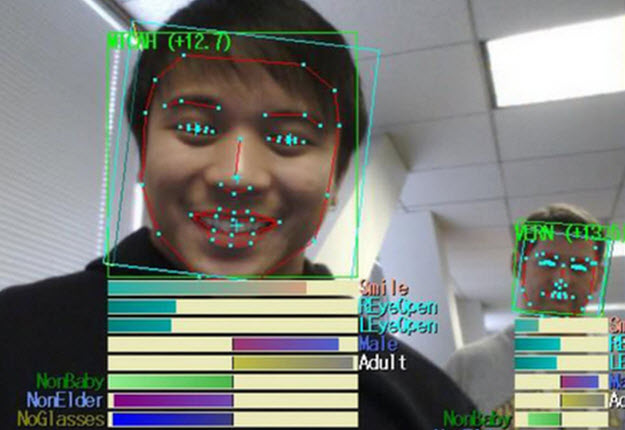
\includegraphics[width=0.8\textwidth]{figures/Face-Recognition}
      \\
      
      {\large A supervised learning problem: object recognition}
    }
    \only<2>{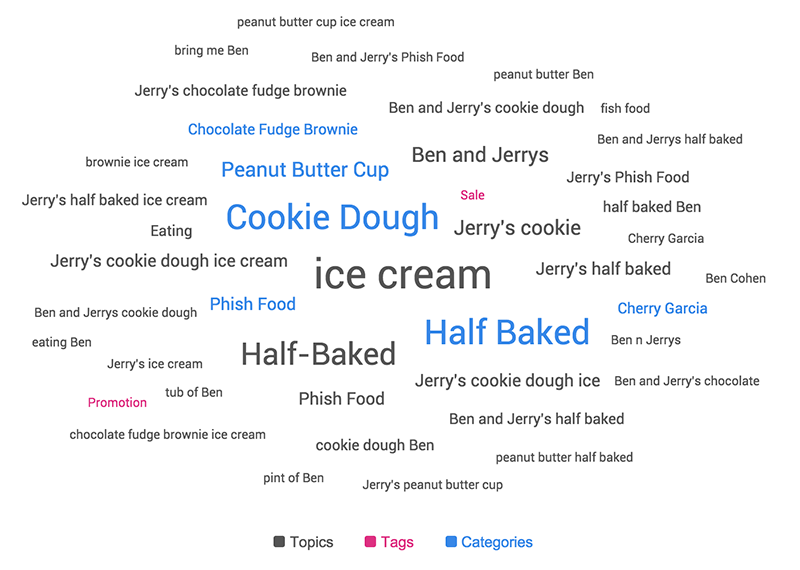
\includegraphics[width=0.8\textwidth]{figures/text-cloud}
      \\
      
      {\large An unsupervised learning problem: topic modelling}
    }

  \end{center}
\end{frame}
\pnote{
  You can use machine learning just to analyse, or find structure in
  the data. This is generally called unsupervised learning. One such
  example is topic modelling, where you let the algorithm find topics
  from a corpus of text.  These days algorithms  are used to learn 
  in many applications.  These include speech recognition, facial
  authentication, weather prediction, etc. In general, in these
  problems we are given a \emph{labelled} dataset with, say, example
  images from each class. Unfortunately this does not scale very
  well, because obtaining labels is expensive.

  This is partially how science works, because what we need to do
  is to find a general rule of nature from data. Starting from some
  hypothesis and some data, we reach a conclusion. However, many
  times we may need to actively experiment to obtain more data,
  perhaps because we found that our model is wrong.
}


\begin{frame}
  \frametitle{Can machines plan ahead?}
  \begin{center}
    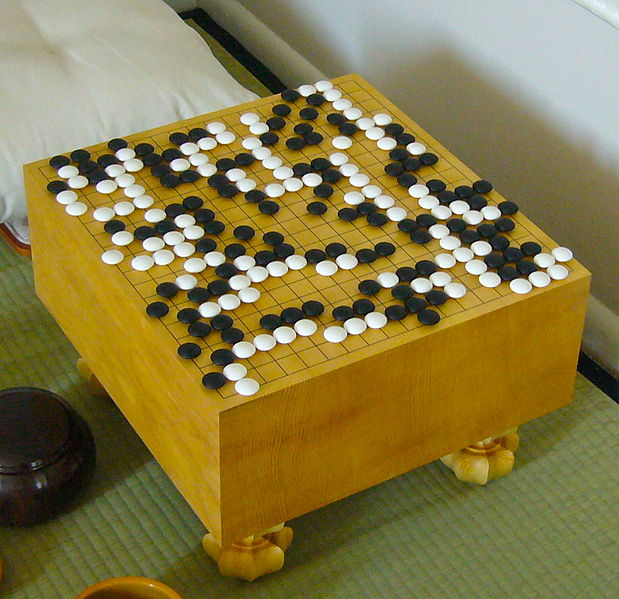
\includegraphics[width=0.8\textwidth]{figures/619px-FloorGoban}
  \end{center}
\end{frame}

\pnote{I suppose the first question for experiment design is whether machines can plan
ahead. Indeed, even for large problems, such as Go, machines can
now perform at least as well as top-rated humans. How is this
 achieved?}


\begin{frame}
  \frametitle{Machines can plan!}
  \begin{center}
    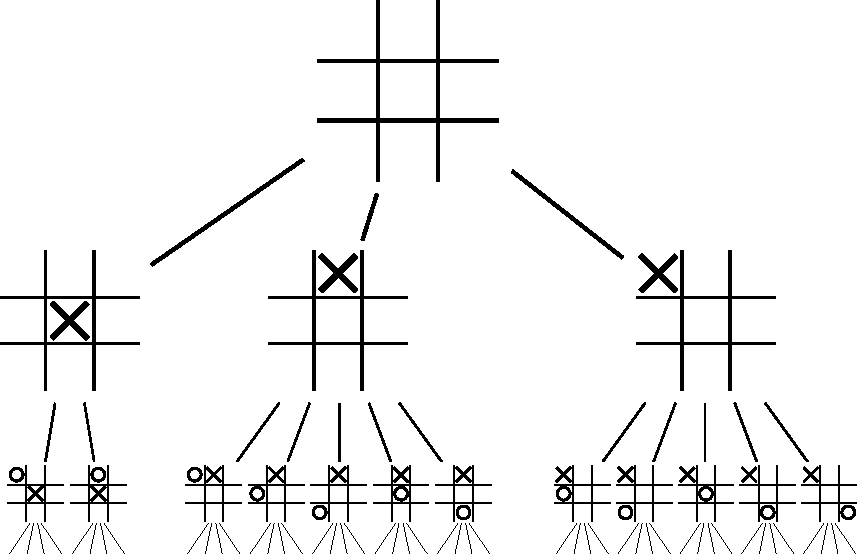
\includegraphics[width=0.8\textwidth]{figures/Tic-tac-toe-game-tree}
  \end{center}
\end{frame}
\pnote{The basic construction is the planning tree. This is an enumeration
of all possible future events. If a complete enumeration is
impossible, a partial tree is constructed. However this requires
evaluating non-terminal game positions. In the past, this was
done with heuristics, but now this is data-driven, both through the
use of expert databases, and through self-play and reinforcement
learning.}


\begin{frame}
  \frametitle{Can machines learn from their mistakes?}
  \begin{center}
    \movie{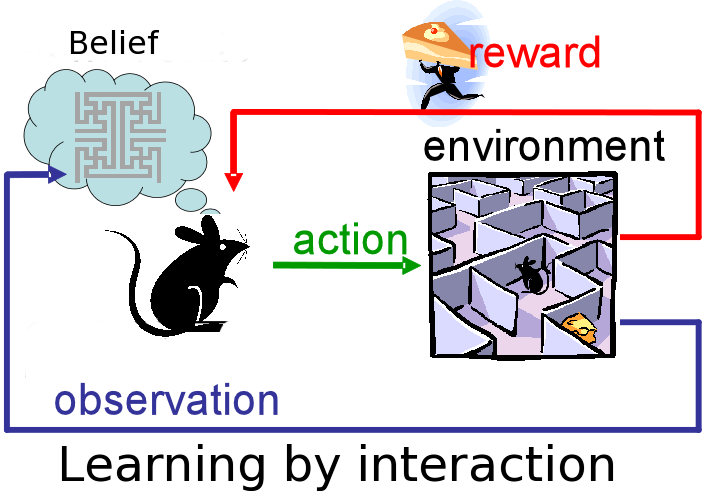
\includegraphics[width=0.75\textwidth]{figures/rl_interaction}}{figures/Pancakes.mp4}
  \end{center}
\end{frame}
\pnote{So, what happens when we make a mistake? Can we somehow recognise
it? Humans and other animals can actually learn from their
mistakes. Consider the proverbial rat in the maze. At some
intervals, the experimenter places some cheese in there, and the
rat must do a series of actions to obtain it, such as navigating
the maze and pulling some levers. It doesn't know how to get to
the cheese easily, but it slowly learns the layout of the maze
through observation, and in the end, through trial-and-error it
is able to get to the cheese very efficiently.

We can formalise this as a reinforcement learning problem, where
the rat takes a series of actions; at each step it also obtains a
reward, let's say equal to 0 when it has no cheese, and 1 when it
eats cheese. Then we can declare that the rat's utility is the sum
of all rewards over time, i.e. the total amount of cheese it can
eat before it dies.

The rat needs to explore the environment in order to be able to
get to the cheese. Here is a robotics example. Let us say that we
are trying to teach a robot to flip pancakes. One easy thing we
can try is to show the robot how to do it, and then let it just
copy the demonstrated movement. However, this doesn't work! The
robot needs to explore variations of the movement, until it
manages to successfully flip pancakes. Again, we can formulate
this as a reinforcement learning problem, with a reward that is
high whenever the pancake's position is flipped, and on the pan;
and low everywhere else. Then the robot can learn to perform this
behaviour through trial and error. It's important to note that in
this example, merely demonstration is not enough. Neither is
reinforcement learning enough. The same thing is true for the
recent success of AlphaGo in beating a master human: apart from
planning, they used both demonstration data and self-play, so that
it could learn through trial and error.
}


\subsection{Automated science}
\begin{frame}
  \centering
  \Huge{The multi-armed bandit}
\end{frame}
\begin{frame}
  \centering
  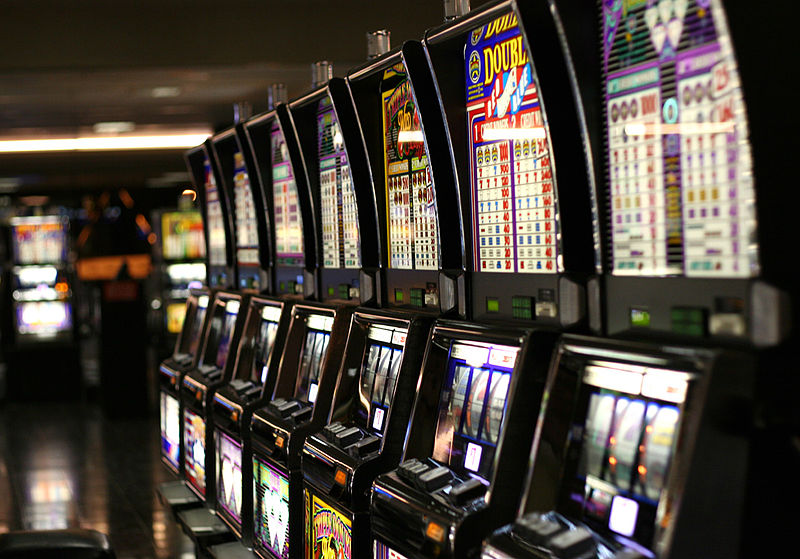
\includegraphics[width=\textwidth]{figures/Las_Vegas_slot_machines}
\end{frame}
\pnote{An example that typifies trial and error learning are bandit
problems. Imagine that you are in a Casino and you wish to
maximise the amount of money you make during the night. There are
a lot of machines to play. If you knew which one was the best,
then you'd just play it all night long. However, you must also
spend time trying out different machines, in order to get an
estimate of how much money each one gives out. The trade off
between trying out different machines and playing the one you
currently think is best is called the exploration-exploitation
trade-off and it appears in many problems of experiment design for
science.}


\begin{frame}
  \frametitle{Adam, the robot scientist}
  \centering
  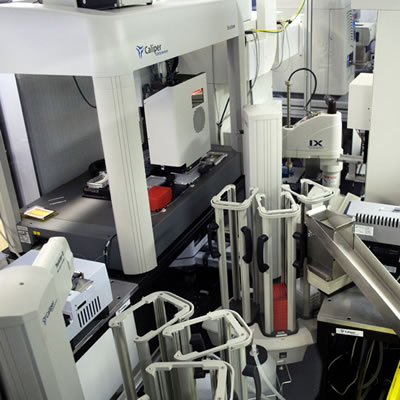
\includegraphics[width=0.8\textwidth]{figures/robot-scientist}
\end{frame}
\pnote{Let's say we want to build a robot scientist and tell it to
discover a cure for cancer. What does the scientist do??}



\begin{frame}
  \frametitle{Active learning for drug discovery}
  \centering
  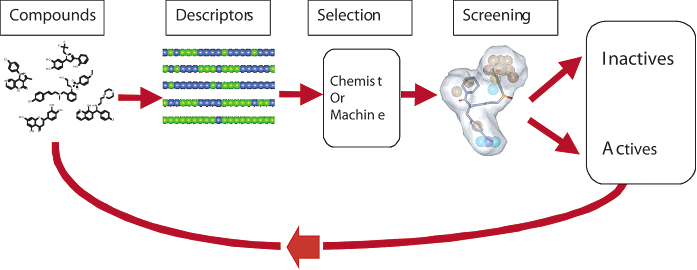
\includegraphics[width=0.9\columnwidth]{figures/drug-discovery-000}
\end{frame}
\pnote{Simplifying the problem a bit, consider that you have a large
number of drug candidates for cancer and you wish to discover
those that are active against it. The ideas is that you select
some of them, then screen them, to sort them into active and
inactive. However, there are too many drugs to screen, so the
process is interactive. At each cycle, we select some drugs to
screen, classify them, and then use this information to select
more drugs to screen. This cycle, consequently has two parts:
1. Selecting some drugs given our current knowledge.
2. Updating our knowledge given new evidence.}

\begin{frame}
  \frametitle{Drawing conclusions from results}
  \centering
  \begin{tikzpicture}[line width=2pt, >={Stealth[length=5mm]}]
    \node at (0,0) (bt) {hypothesis};
    \node[select] at (0,2) (at) {experiment};
    \node[utility] at (3,-2) (rt) {result};
    \draw[blue,->] (at) -- (rt);
    \node at (4,0) (bt2) {conclusion};
    \draw[red,->] (at) -- (bt2);
    \draw[red,->] (bt) -- (bt2);
    \draw[red,->] (rt) -- (bt2);
  \end{tikzpicture}
\end{frame}
\pnote{  In general, we would like to have some method which can draw
  conclusions from results. This involves starting with a
  hypothesis, performing an experiment to verify or refute it,
  obtain some experimental result; and then concluding for or
  against the hypothesis. Here the arrows show dependencies
  between these variables. So what do we mean by "hypothesis" in this case?
  }

\begin{frame}
  \frametitle{Tycho Brahe's minute eye measurements}
  \begin{columns}
    \begin{column}{0.4\textwidth}
      \uncover<4->{
        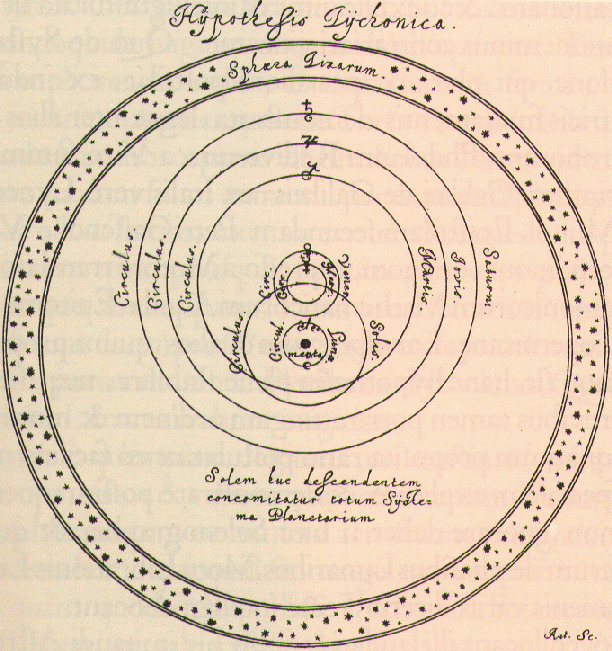
\includegraphics[width=\columnwidth]{figures/circular-orbits}
      }
    \end{column}
    \begin{column}{0.5\textwidth}
      \uncover<2->{
        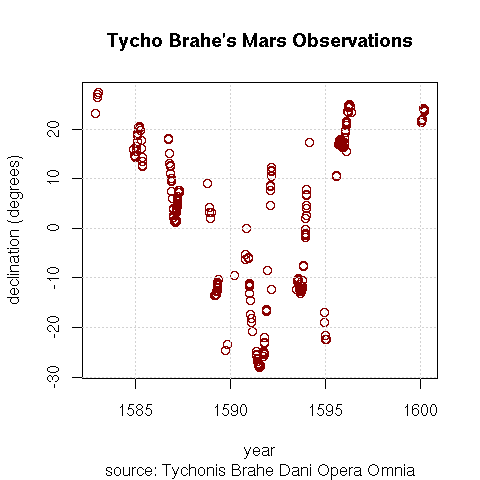
\includegraphics[width=\columnwidth]{figures/tycho-observations}
      }
    \end{column}
  \end{columns}
  \begin{columns}
    \begin{column}{0.1\textwidth}
      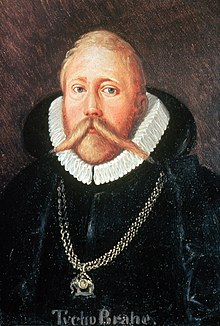
\includegraphics[width=4em]{figures/Tycho-Brahe.jpg}
    \end{column}
    \begin{column}{0.9\textwidth}
      \begin{itemize}
      \item<3-> Hypothesis: \alert{Circular} orbits around the \alert{earth}
      \item<4-> Conclusion: \alert{Specific} circular orbits around the earth
      \end{itemize}
    \end{column}
  \end{columns}
\end{frame}
\pnote{Let's take the example of planetary orbits. Here Tycho famously
 spent 20 years experimentally measuring the location of Mars. He
 had a hypothesis: that planetary orbits were circular, but he
 didn't know which were the right orbits. When he tried to fit his data to this hypothesis, he concluded a specific circular orbit for Mars... around Earth.}

\begin{frame}
  \frametitle{Johannes Kepler's alternative hypothesis}
  \begin{columns}
    \begin{column}{0.5\textwidth}
      \uncover<4->{
        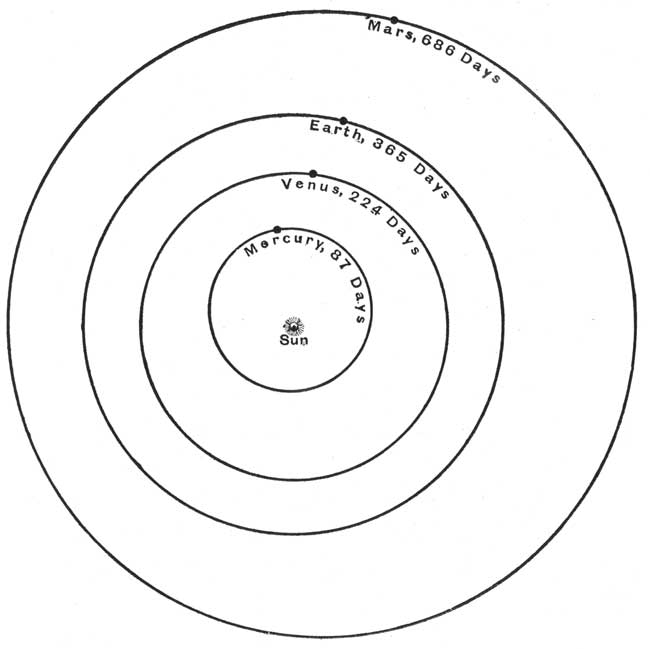
\includegraphics[width=\columnwidth]{figures/orbits}
      }
    \end{column}
    \begin{column}{0.5\textwidth}
      \uncover<2->{
        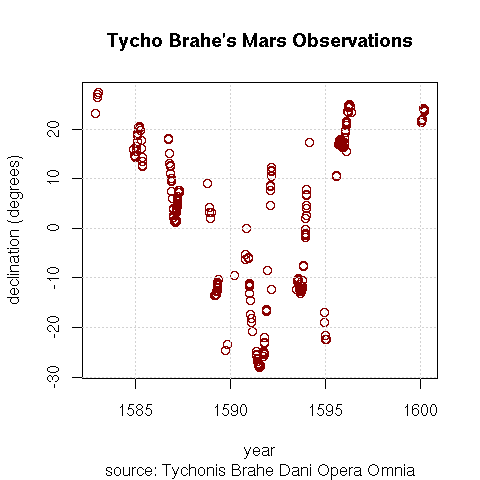
\includegraphics[width=\columnwidth]{figures/tycho-observations}
      }
    \end{column}
  \end{columns}
  \begin{columns}
    \begin{column}{0.1\textwidth}
      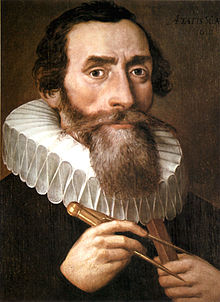
\includegraphics[width=4em]{figures/Johannes-Kepler.jpg}
    \end{column}
    \begin{column}{0.9\textwidth}
      \begin{itemize}
      \item<3-> Hypothesis: Circular \alert{or} elliptic orbits around the \alert{sun}
      \item<4-> Conclusion: Specific \alert{elliptic} orbits
      \end{itemize}
    \end{column}
  \end{columns}
\end{frame}

\pnote{Kepler had a more general hypothesis: that orbits could be
circular or elliptic. This led him to the broadly correct model
of all planets being in elliptical orbits around the
sun. However, the actual verification that all things do not revolve around earth, requires different experiments.
}
\begin{frame}
  \frametitle{200 years later, Gauss formalised this statistically}
  \begin{columns}
    \begin{column}{0.5\textwidth}
      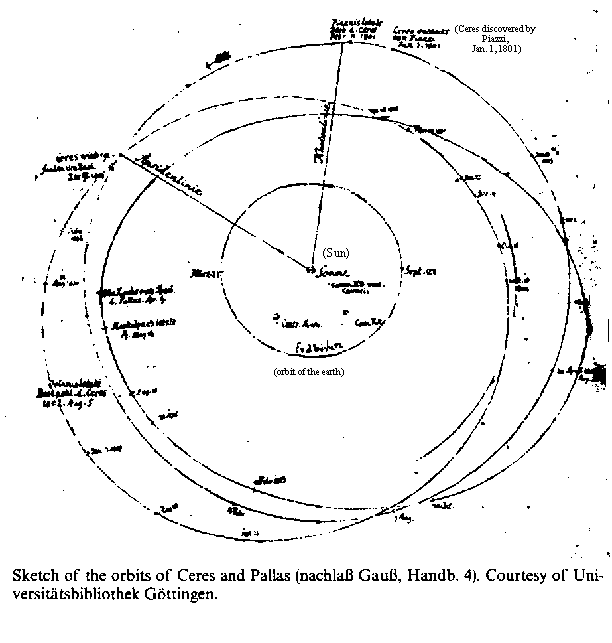
\includegraphics[width=\columnwidth]{figures/gauss-diagram}
    \end{column}
    \begin{column}{0.5\textwidth}
      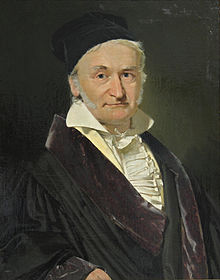
\includegraphics[width=4em]{figures/Gauss.jpg}
      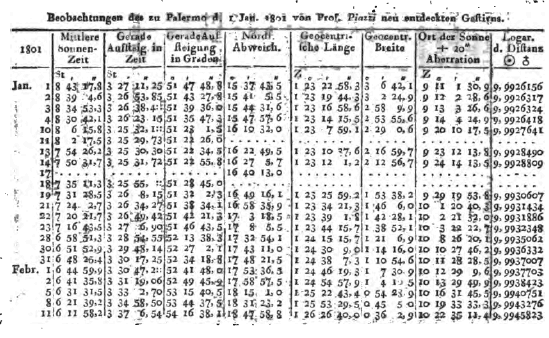
\includegraphics[width=\columnwidth]{figures/SeptemberTable}
    \end{column}
  \end{columns}
\end{frame}
%%% Later on, Gauss collected even more experimental data to calculate the orbit of Ceres. He did this using one of the first formal statistical methods; this allowed him to avoid cheating (like Kepler did, to accentuate his finding that orbits were elliptical).

\begin{frame}
  \frametitle{Statistical visualisation: fMRI}
  \centering
  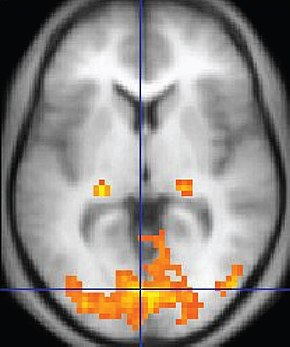
\includegraphics[width=0.5\textwidth]{figures/brain-fmri}
\end{frame}

\begin{frame}
  \frametitle{A warning: The dead salmon mirage}
  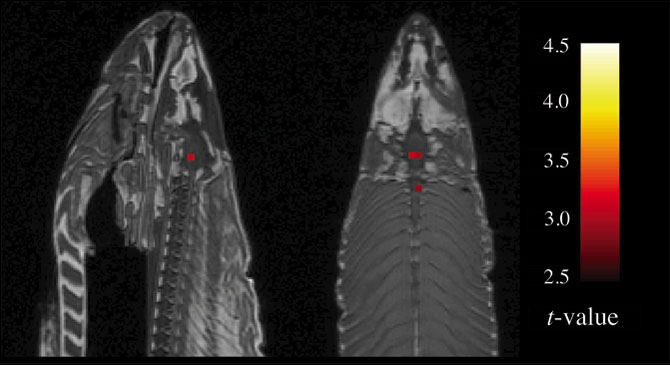
\includegraphics[width=\textwidth]{figures/fmri-salmon}
\end{frame}
\pnote{ It is quite easy to draw the wrong conclusions from
  applying machine learning / statistics to your data. For example, it
  was fashionable to perform fMRI studies in humans to see whether
  some neurons have a particular functional role. So some scientists
  tried to replicate those results. They took a dead salmon, and put
  it an fMRI scanner. They checked its brain activity when it was
  shown images of happy or sad people. Perhaps surprisingly, they
  found an area of the brain that was correlated with the pictures -
  so it seemed, as though the dead salmon could distinguish photos of
  happy people from sad ones. However, this was all due to a
  misapplication of statistics. In this course, we will try and teach
  you to avoid such mistakes.  }


\begin{frame}
  \frametitle{Planning future experiments}
  \centering
  \begin{tikzpicture}[line width=2pt, >={Stealth[length=5mm]}]
    \node at (0,0) (bt) {hypothesis};
    \node[select] at (0,2) (at) {experiment};
    \node[utility] at (3,-2) (rt) {result};
    \draw[blue,->] (at) -- (rt);
    \node at (4,0) (bt2) {conclusion};
    \draw[red,->] (at) -- (bt2);
    \draw[red,->] (bt) -- (bt2);
    \draw[red,->] (rt) -- (bt2);
  \end{tikzpicture}
\end{frame}
%%% I mentioned before that we must decide what experiment to do. This is indeed difficult, especially in setting such as drug discovery where the number of experiments is huge. 


\begin{frame}
  \frametitle{Planning experiments is like Tic-Tac-Toe}
  \begin{center}
    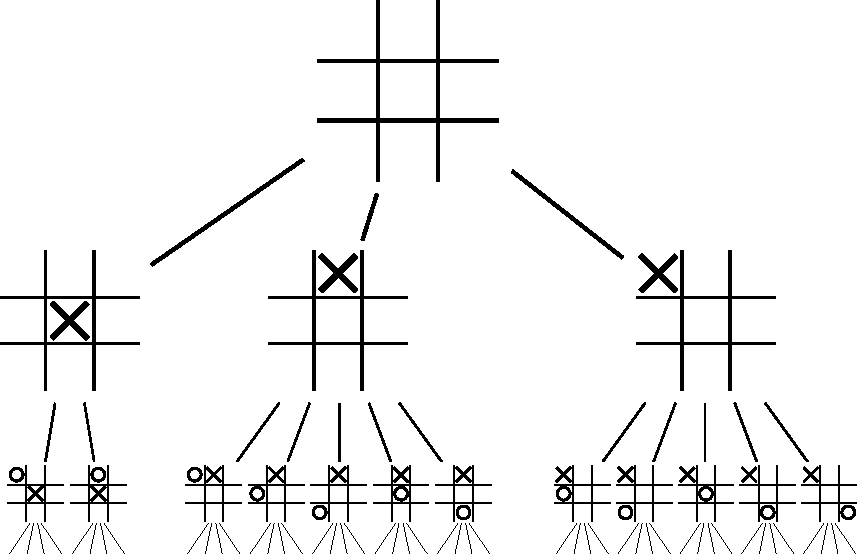
\includegraphics[width=\textwidth]{figures/Tic-tac-toe-game-tree}
  \end{center}
\end{frame}
%%% The basic idea is to think of experiment design as a game between the scientist and Nature. At every step, the scientist plays an X to  denote an experiment. Then Nature responds with an Observation. The main difference is that Nature is probably not adversarial.

\begin{frame}
  \frametitle{Eve, another robot scientist}
  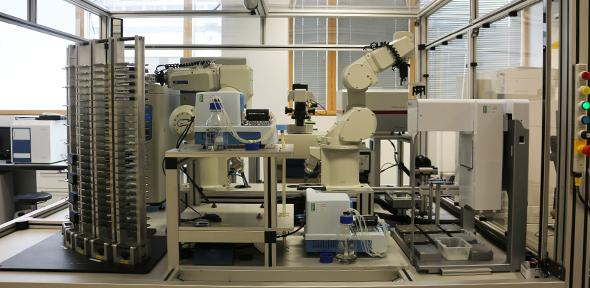
\includegraphics[width=\textwidth]{figures/eve.jpg}
  Discovered a malaria drug
\end{frame}
%%% These kinds of techniques, coming from the multi-armed bandit literature have been successfully used at the university of Manchester to create a robot that recently (re)-discovered a malaria drug.

\section{Societal issues}
\begin{frame}
  \frametitle{Pervasive ``intelligent'' systems}
  \begin{columns}
    \begin{column}{0.3\textwidth}
      \centering
      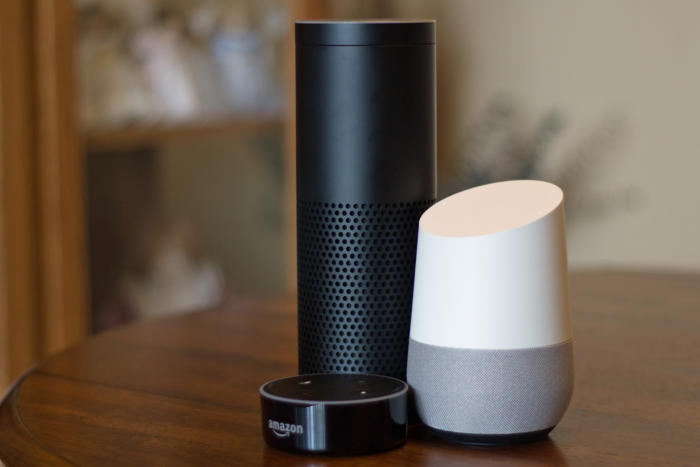
\includegraphics[width=\textwidth]{figures/echo-home.jpg}
      \\
      Home assistants

      \vspace{\fill}

      \bigskip

      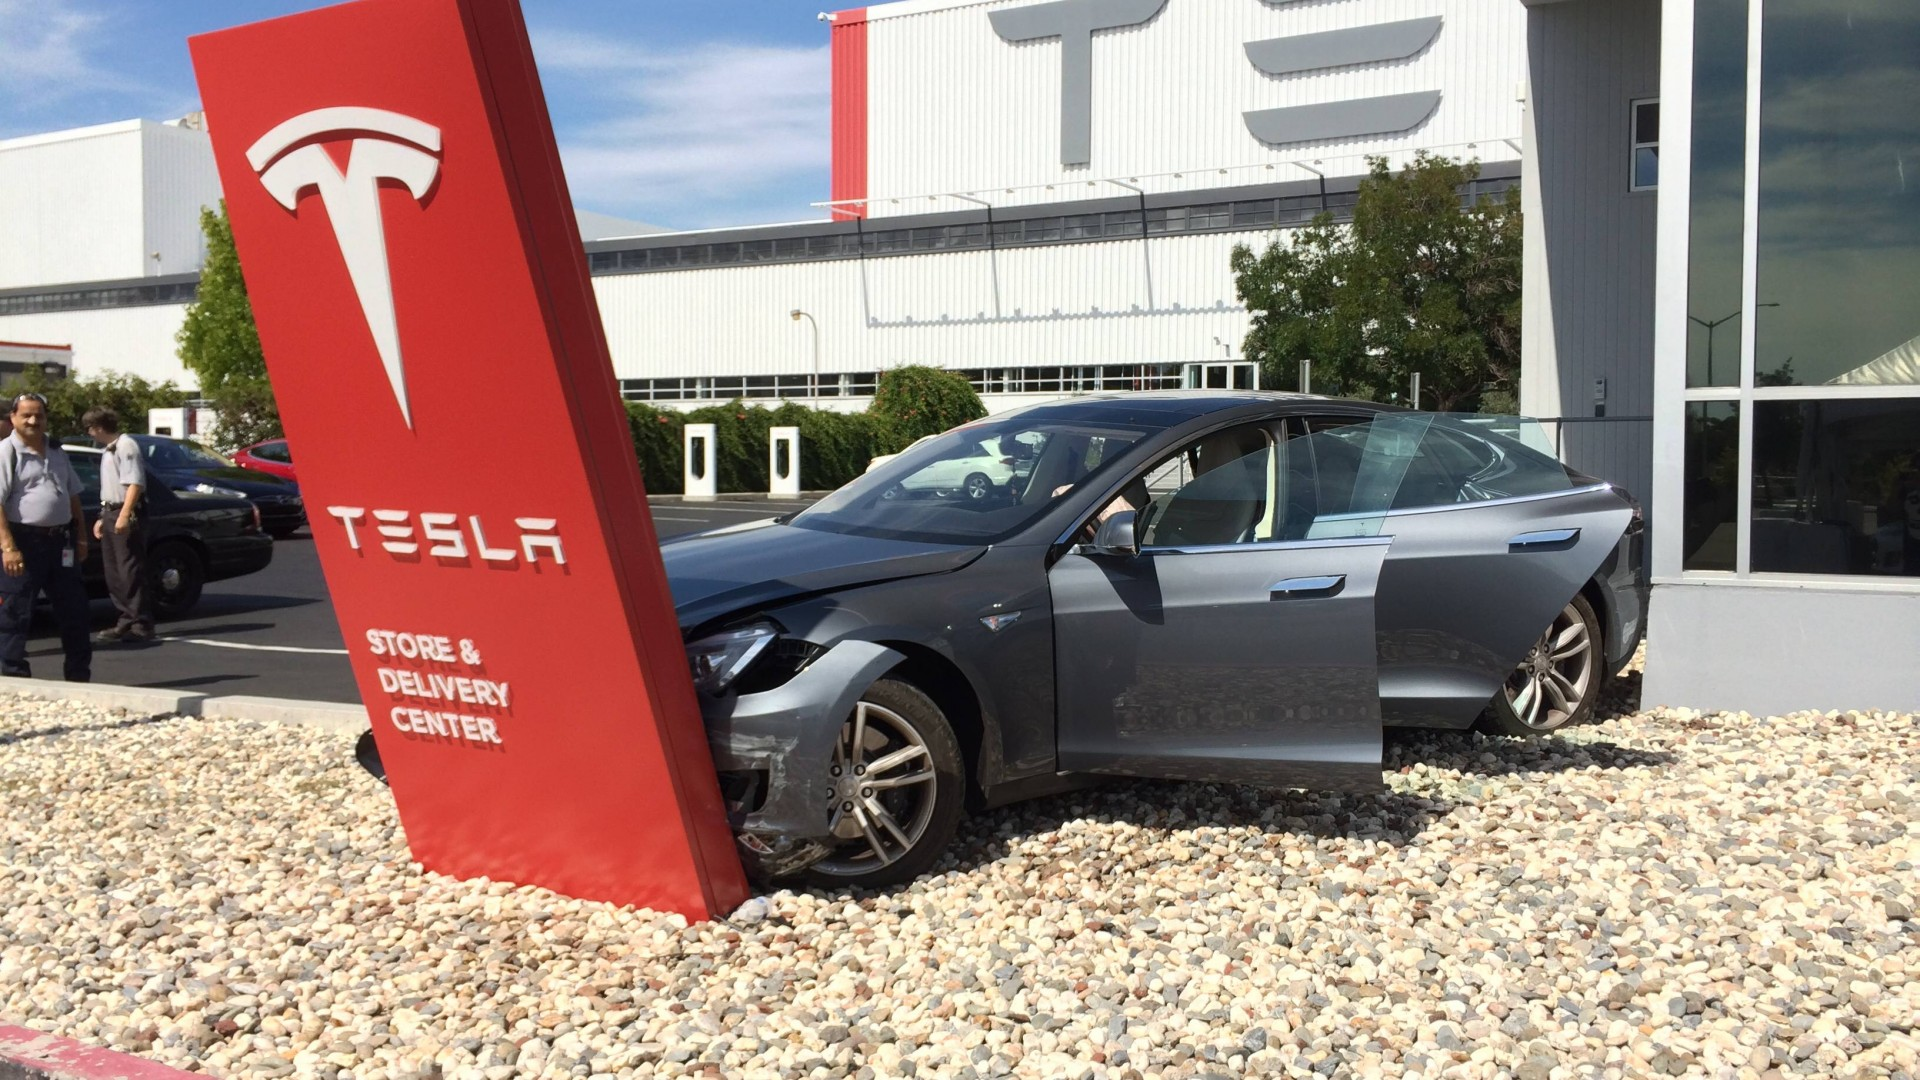
\includegraphics[width=\textwidth]{figures/tesla.jpg}
      \\
      Autonomous vehicles
    \end{column}
    \begin{column}{0.3\textwidth}
      \centering 
      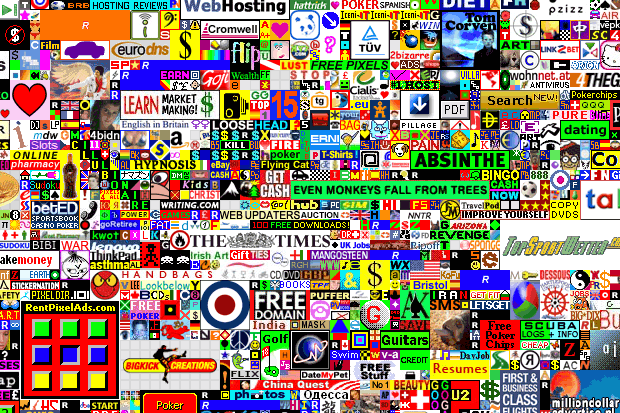
\includegraphics[width=\textwidth]{figures/web-ads.png}
      \\
      Web advertising

      \vspace{\fill}

      \bigskip

      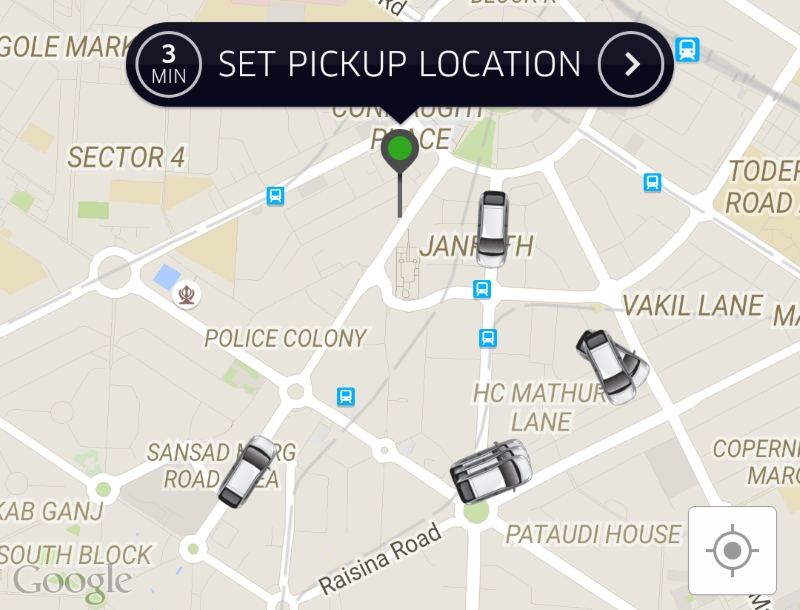
\includegraphics[width=\textwidth]{figures/uber-here-maps.jpg}
      \\
      Ridesharing
    \end{column}
    \begin{column}{0.3\textwidth}
      \centering 
      \\
      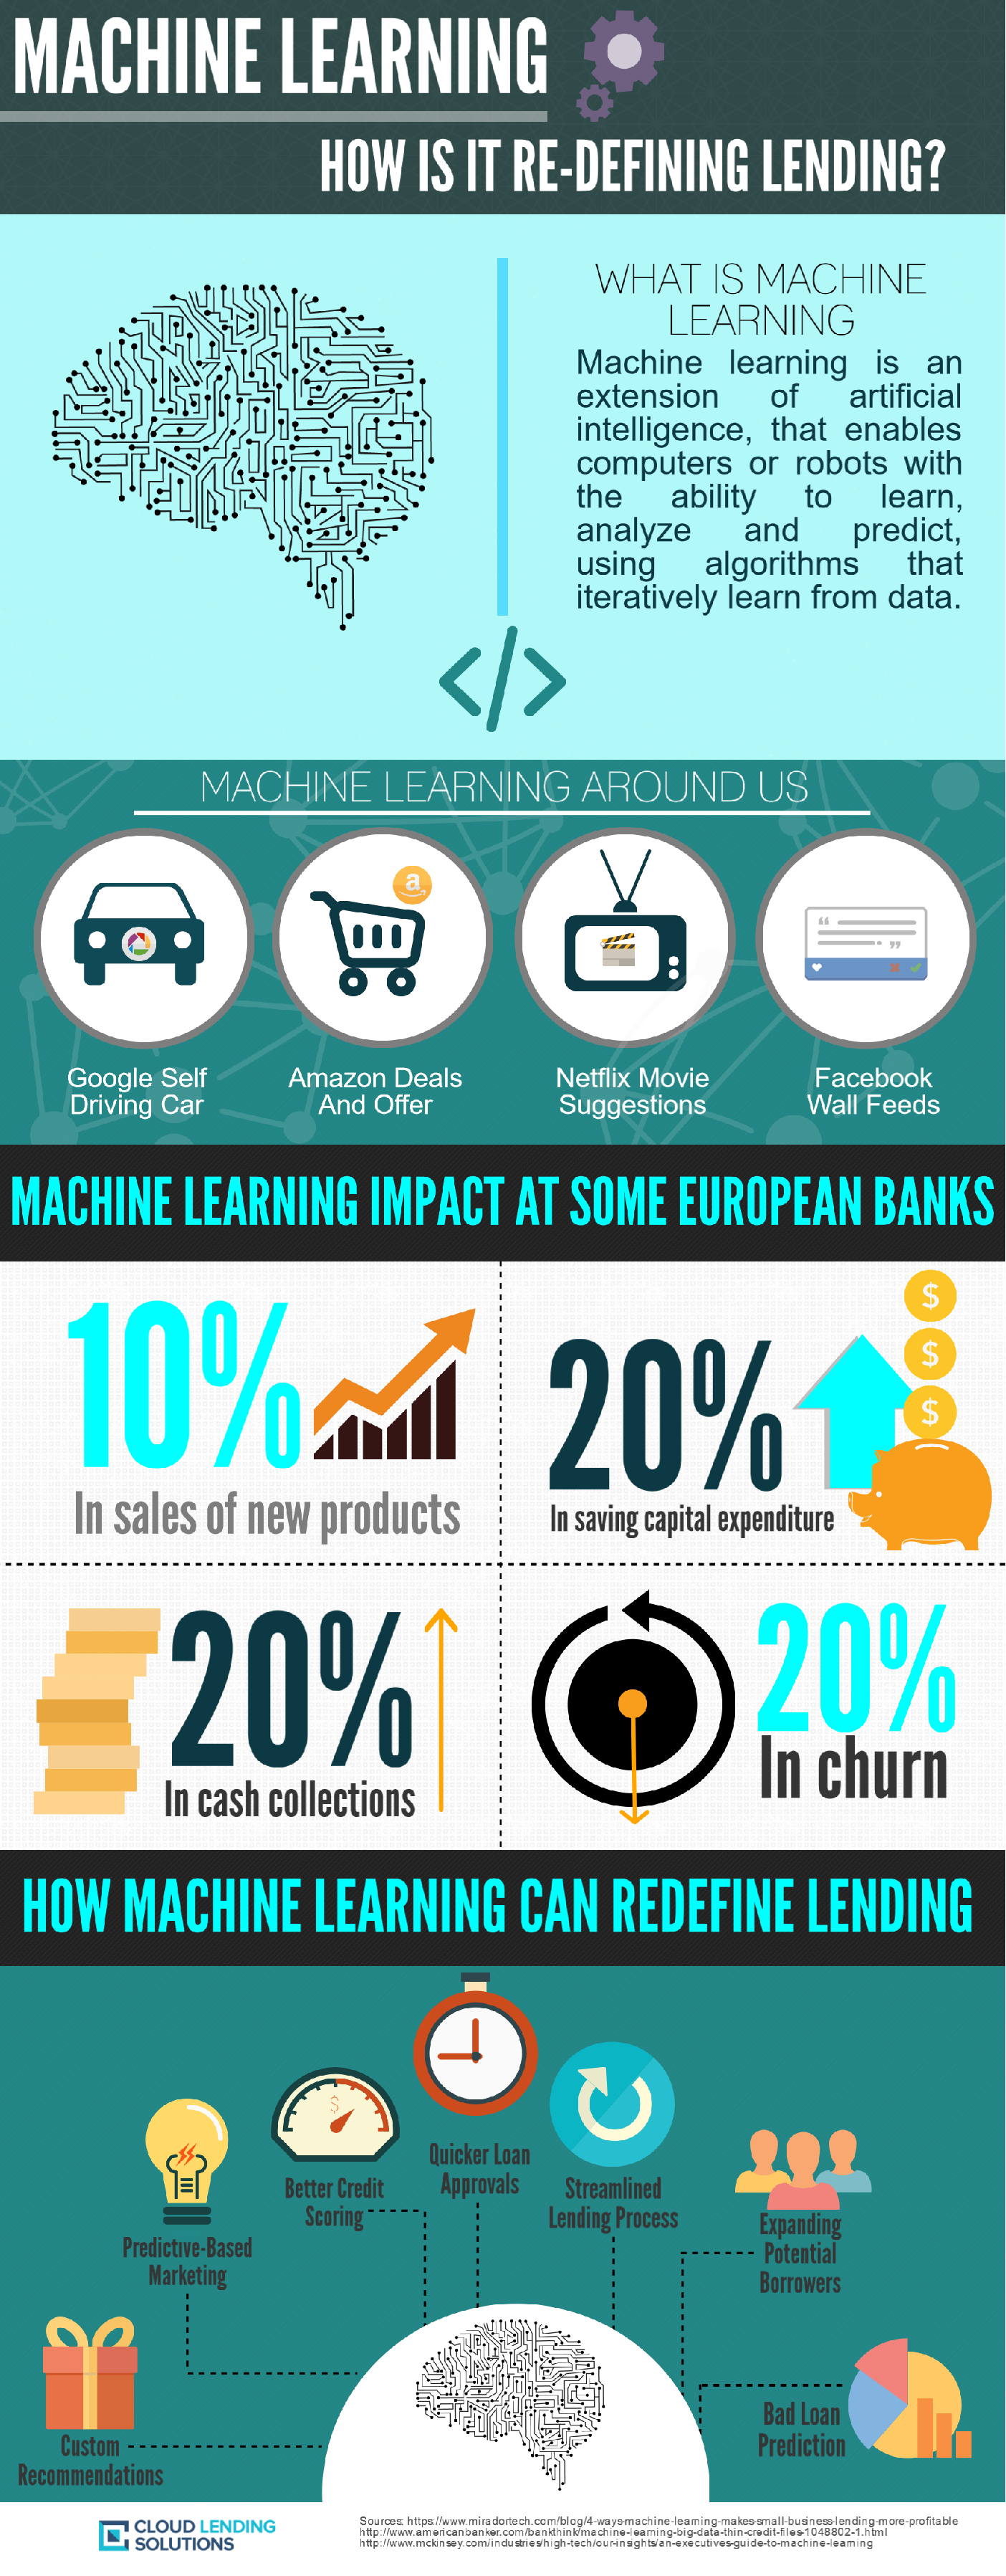
\includegraphics[width=\textwidth,clip = true, trim=0 0 0 42.5cm]{figures/lending.pdf}
      \\
      Lending

      \vspace{\fill}

      \bigskip

      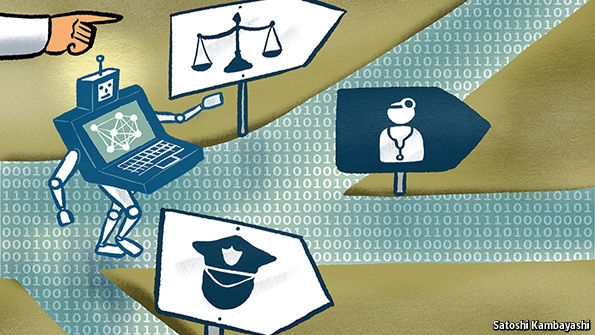
\includegraphics[width=\textwidth]{figures/algorithms-public.jpg}
      \\
      Public policy
    \end{column}
  \end{columns}
  \only<2>{
    \begin{tikzpicture}[remember picture,overlay]
      \draw[fill=black,opacity=0.75] 
      (current page.north east) rectangle (current page.south west);
      \node at (current page.center) {
        {\Huge \alert{Privacy, Fairness, Safety}}
      };
    \end{tikzpicture}}
  \pnote{Artificial intelligence is no longer limited to scientific applications and classical problems in AI such as playing games. AI is now deployed at large scale. These range from simple recommendation systems such as home assistants gather information about our habits, showering us with targeted ads and financial services; or more complex systems such as semi-autonomous vehicles. AI systems are also used increasing to direct human lives: ridesharing is an easy example, as drivers obtain instructions from an automated system. A less-known example is that AI now also shapes public policy. Automated policing, medical diagnostics and justice, are three cases in point.}
\pnote{Even if we assume these systems are well-designed, they have many negative implications. The first is privacy. In order to enable these technologies, some personal data must be collected. What guarantees do we have about how the data is used and what type of personal information can be leaked? The second is fairness. If a ridesharing app replaces standard taxis and buses, would this result in degraded transport services in poor areas of town? Would our CV screening application routinely turn down excellent female applicants? Finally, what can we say about the safety, i.e. the tail risks of technologies such as self-driving cars?}
\end{frame}

%%% Local Variables:
%%% mode: latex
%%% TeX-master: "basel-presentation"
%%% End:




\end{document}

%%% Local Variables:
%%% mode: latex
%%% TeX-master: t
%%% End:
